\section{Cartesian Space Impedance Control}\label{sec:hsacontrol:operational_space_impedance_control}
We introduce below a novel control strategy that addresses some limitations of the configuration-space regulation controller presented in Sec.~\ref{sub:hsacontrol:configuration_space_regulation:control_strategy} that are critical for achieving both structural and computational compliance. Namely, we (i) avoid computationally demanding planning procedures, (ii) remove integral terms that are unsafe for environment interaction, and (iii) enable impedance shaping in operational space. This Cartesian-space impedance controller is inspired by \citep{ott2008cartesian} and \citep{della2020model}, but specifically designed for and tailored to \gls{HSA} robots. Crucially, we need to overcome the challenges of underactuation and the nonlinearity in the actuation, which were not present in that original work. %We, therefore, solve online a least-squares optimization problem, identifying the optimal actuation for generating the demanded operational space forces.

\begin{figure}
    \centering
    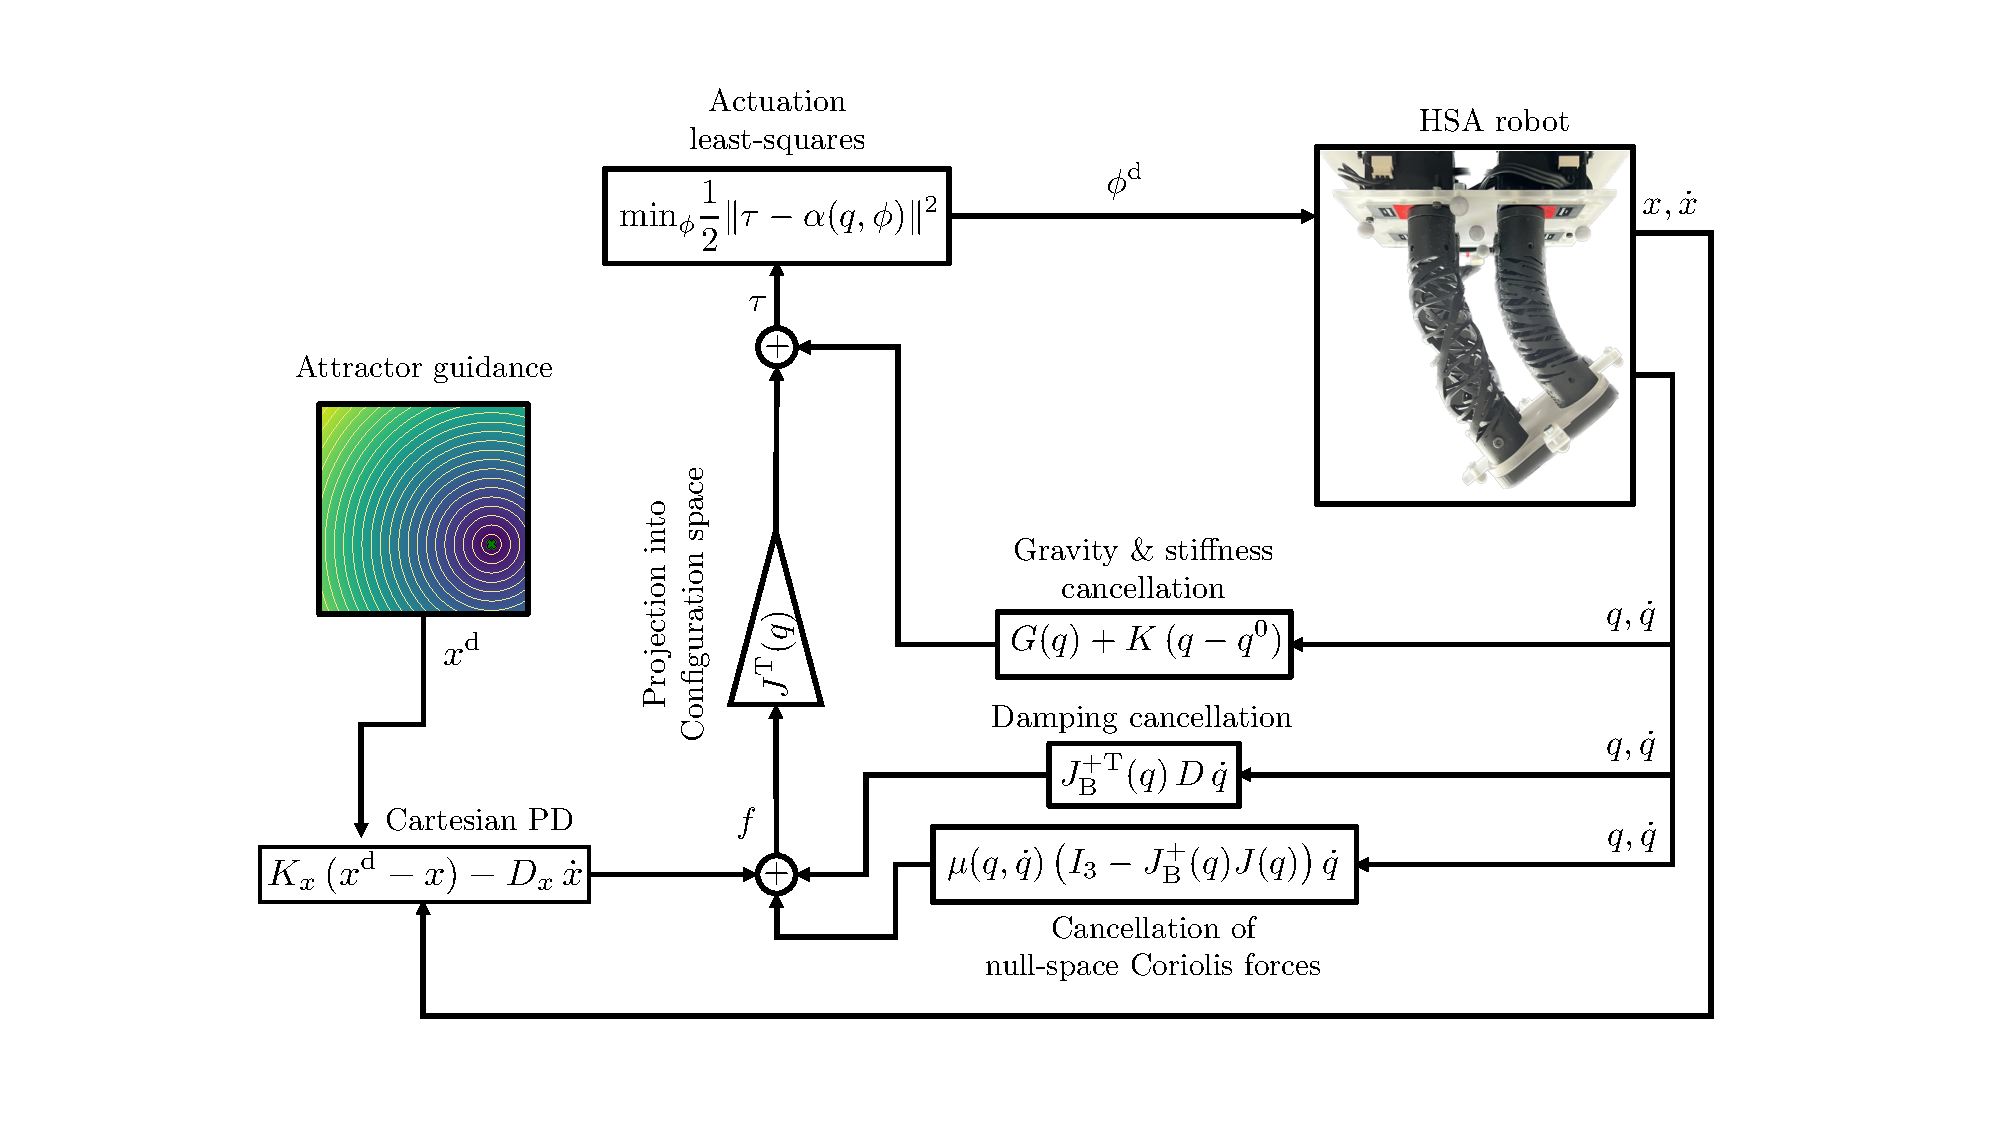
\includegraphics[width=0.9\textwidth]{hsacontrol/figures/control_schemes/cartesian_impedance_control/control_scheme_without_brain_control_cropped.pdf}
    \caption{Block scheme of the operational space space impedance controller: after the cancellation of the existing soft robot dynamics (e.g., null-space Coriolis forces, gravity, stiffness, and damping), we reshape the potential field according to the desired Cartesian impedance $K_x, D_x$ with a globally asymptotically stable equilibrium at $x=x^\mathrm{d}$. Subsequently, we project the desired forcing $f$ from operational space to configuration space. Finally, we solve a nonlinear least-squares optimization problem to match the desired configuration-space torques $\tau$ as closely as possible with the torques generated by the actuation $\phi^\mathrm{d}$.}
    \label{fig:hsacontrol:task_space_impedance_control:block_scheme_closed_loop_control}
\end{figure}

\subsection{Background: Operational Space Dynamics}\label{sub:hsacontrol:task_space_dynamics}
%
Although this has never been done in the context of HSA robots, it is immediate to see that their dynamics \eqref{eq:hsacontrol:dynamics} can be projected into operational space, yielding the form~\citep{della2019exact, della2020model} % khatib1987unified
\begin{equation}\label{eq:hsacontrol:operational_space_dynamics}
    \Lambda(q) \, \Ddot{x} + \mu(q,\dot{q}) \dot{q} + J_\mathrm{M}^{+\top} ( G(q) + K (q-q^0) + D \, \dot{q} ) = J_\mathrm{M}^{+\top} \alpha(q,\phi),
\end{equation}
where $J_\mathrm{M}^+(q) = M^{-1} J^\top(J M^{-1} J^\top)^{-1} \in \mathbb{R}^{3\times2}$ is the dynamically consistent pseudo-inverse, $\Lambda(q) = (J \, M^{-1} J^\top)^{-1} \in \mathbb{R}^{2 \times 2}$ is the inertia matrix in operational space, and $\mu(q, \dot{q}) = \Lambda(q) \, (J M^{-1} C - \dot{J}) \in \mathbb{R}^{2 \times 3}$ collects the Cartesian Coriolis and centrifugal terms. % ~\citep{khatib1987unified}

\subsection{Control Strategy}\label{sub:hsacontrol:task_space_impedance_control:control_strategy}
% In previous work~\citep{stolzle2024experimental}, we have devised a model-based control strategy for regulating a planar \gls{HSA} robot towards a desired position in operational space. %We propose here a new strategy that overcomes several limitations of that previous work which are critical for the application discussed in this chapter - namely: (i) it involves a complex and computationally demanding planning procedure for identifying a suitable setpoint in configuration space, (ii) our configuration-space controller contains integral terms, making it unsafe for environment interactions, and (iii) it is based on a compensation of static forces in configuration-space thus not allowing us to shape the impedance characteristics in operational space.
%
We will present the control strategy in two steps: first, we will introduce the control law and derive the associated desired configuration-space torques, and second, we will discuss how to map the control inputs to the actuation $\phi$.

\subsubsection{Proposed Controller}
% We implement an operational space impedance action~\citep{ott2008cartesian, della2020model} that renders $x^\mathrm{d}$ an attractor of the closed-loop system.
We propose the following dynamic feedback law that renders $x^\mathrm{d}$ an attractor of the closed-loop system %~\citep{ott2008cartesian, della2020model} 
\begin{equation}\label{eq:hsacontrol:task_space_impedance_control:cartesian_impedance_controller}
\begin{split}
    \tau =& \: J^\top(q) \, \left (K_x \, (x^\mathrm{d} - x) - D_x \, \dot{x} \right ) + G(q) + K \, (q-q^0)\\
    & \: + J^\top(q) \, J_\mathrm{M}^{+\top}(q) \, D \, \dot{q} + J^\top(q) \, \mu(q,\dot{q}) \left ( \mathbb{I}_3 - J_\mathrm{M}^+(q) J(q) \right )\dot{q}
\end{split}
\end{equation}
where $\tau \in \mathbb{R}^3$ is the desired torque in configuration space, $G(q) + K \, (q-q^0)$ cancels the acting gravitational and elastic forces, and $J^\top J_\mathrm{M}^{+\top} D \, \dot{q}$ removes the natural dissipation in operational space.
We emphasize that because the system is underactuated, we need to cancel the stiffness directly in the configuration instead of operational space as done in previous work~\citep{della2020model}.
We can shape our desired impedance characteristics in Cartesian space with the PD term $f_\mathrm{PD} = K_x \, (x^\mathrm{d} - x) - D_x \, \dot{x} $ which is then projected into configuration space by premultiplying with $J^\top(q)$.

The term $\mu(q,\dot{q}) \left ( \mathbb{I}_3 - J_\mathrm{M}^+(q) J(q) \right )\dot{q}$ decouples the operational space dynamics from the residual of the null-space dynamics~\citep{ott2008cartesian, della2020model}. % \cite[Ch. 4]{ott2008cartesian}.
The identity $\dot{q} = J_\mathrm{M}^+ \, \dot{x} + Z^\top \, \nu_\mathrm{N}$, where $Z^\top \in \mathbb{R}^{3 \times 1}$ is the dynamically-consistent pseudo-inverse of the null space, allows us to formulate $\dot{q}$ as a sum of the operational space velocity $\dot{x}$ and the null-space velocity $\nu_\mathrm{N}$. Leveraging this identity, the Coriolis and centrifugal matrix $\mu(q,\dot{q})$ can be split into a term $\mu_x(q,\dot{q}) = \mu \, J_\mathrm{M}^+ \in \mathbb{R}^{2 \times 2}$ excited by $x$ and the expression $\mu_\mathrm{N}(q,\dot{q}) = \mu \, Z^\top \in \mathbb{R}^{2 \times 1}$ that is excited by the null-space coordinates resulting in $\mu(q,\dot{q}) \, \dot{q} = \mu_x(q,\dot{q}) \, \dot{x} + \mu_\mathrm{N}(q,\dot{q}) \, \nu_\mathrm{N}$.
This allows us to cancel the term $\mu_\mathrm{N}(q,\dot{q}) \, \nu_\mathrm{N}$ through $\mu(q,\dot{q}) \left ( \mathbb{I}_3 - J_\mathrm{M}^+(q) J(q) \right )\dot{q}$ without having to compute the null space explicitly.


% The first step consists of establishing a PD feedback in Cartesian space
% \begin{equation}
%     f =  K_x \, (x^\mathrm{d} - x) - D_x \, \dot{x} + J_\mathrm{M}^{+\top} \, D \, \dot{q}. % + \eta(q, \dot{q}) J_\mathrm{M}^+ \left (G(q) + K \, q \right ).
% \end{equation}
% where $K_x \in \mathbb{R}^{2\times2}$ is the designed operational space stiffness and $D_x % \in \mathbb{R}^{2\times2}$ adds dissipation.
% We make use of the kinematic Jacobian to project the designed operational space force into % configuration space and additionally establish cancellation of the gravitational and % elastic forces with
% \begin{equation}
%     \tau = \alpha(q,\phi) = J^\top(q) \, f + G(q) + K \, (q-q^0).
% \end{equation}

In summary, the closed-loop dynamics in operational space can be stated as
\begin{equation}\label{eq:hsacontrol:task_space_impedance_control:closed_loop_dynamics}
    \Lambda(q) \, \Ddot{x} + \mu(q,\dot{q}) \, J_\mathrm{M}^+ \, \dot{x} + K_x \, (x^\mathrm{d} - x) - D_x \, \dot{x} = 0,
\end{equation}
which results in $x^\mathrm{d}$ being the globally asymptotically stable equilibrium of the operational space dynamics.


\subsubsection{Mapping to Actuation}
%
Now that we have formulated our control law $\tau$ in configuration space, we need to identify a strategy to specify the motor angles $\phi \in \mathbb{R}^2$ such that $\alpha(q,\phi) \approx \tau$. Note that, in contrast to other continuum soft robots studied in literature~\citep{della2023model}, the actuation term $\alpha(q,\phi)$ is not affine in control. %, but rather a nonlinear function with respect to the actuation coordinates $\phi$. 
%Therefore, mapping configuration-space torques to motor commands is not straightforward.
In previous work~\citep{stolzle2024experimental}, we side-stepped this challenge by linearizing with respect to the steady-state actuation $\phi^\mathrm{ss}$: $A(q) = \lVert \frac{\partial \alpha}{\partial \phi}\rVert_{\phi=\phi^\mathrm{ss}}$ therefore recovering the usual scenario of an affine actuation function. Unfortunately, this is not possible in the setting of this work as i) we do not have access to such $\phi^\mathrm{ss}$, and ii) linearizing around $\phi$ causes the closed-loop system to become unstable. We, therefore, propose to formulate instead a nonlinear least-squares problem $\phi^\mathrm{d} = \argmin_\phi \frac{1}{2} \lVert \tau - \alpha(q,\phi) \rVert^2$ and solve it in real-time with a Levenberg Marquardt solver implemented in JAX~\citep{jaxopt_implicit_diff}.

We note that this approach is not guaranteed to be valid for the general case of an underactuated soft robot but for this particular structure of $\alpha(q,\phi) \in \mathbb{R}^3$ with $\phi \in \mathbb{R}^2$ it is possible to identify solutions $\phi$ with the Euclidean norm of the residual being smaller than $0.001$.
The source code of the controller is available on GitHub\footnote{\url{https://github.com/tud-phi/hsa-planar-control}}.
% Next, the actuation vector is linearized with respect to the current twist angle $A_\phi(q) = \frac{\partial \alpha}{\partial \phi} \big|_{\phi} \in \mathbb{R}^{3 \times 2}$. With that, we now have
% \begin{equation}
%     J^\top f = \alpha(q,\phi) + A_\phi(q) \, u
% \end{equation}

\begin{figure}[t]
    \centering
    \subfigure[End-effector x-coordinate]{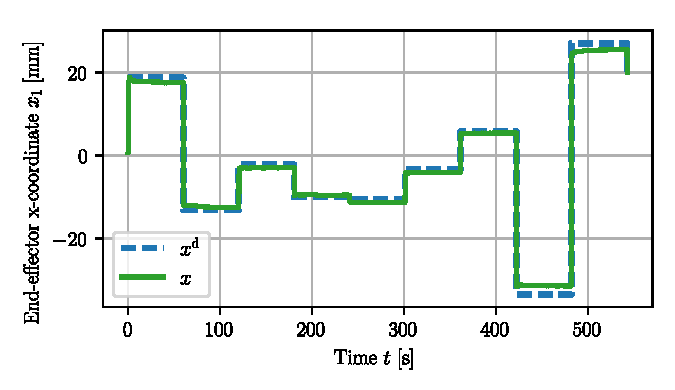
\includegraphics[width=0.47\textwidth, trim={5, 5, 5, 5}]{hsacontrol/figures/experimental_results/task_space_impedance_control/20231030_181558_pee_x.pdf}\label{fig:hsacontrol:experimental_results:task_space_impedance_control:pee_x}}
    \subfigure[End-effector y-coordinate]{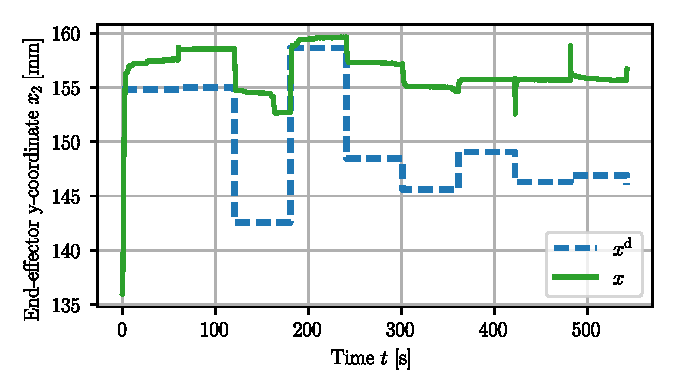
\includegraphics[width=0.47\textwidth, trim={5, 5, 5, 5}]{hsacontrol/figures/experimental_results/task_space_impedance_control/20231030_181558_pee_y.pdf}\label{fig:hsacontrol:experimental_results:task_space_impedance_control:pee_y}}\\
    \subfigure[Configuration $q$]{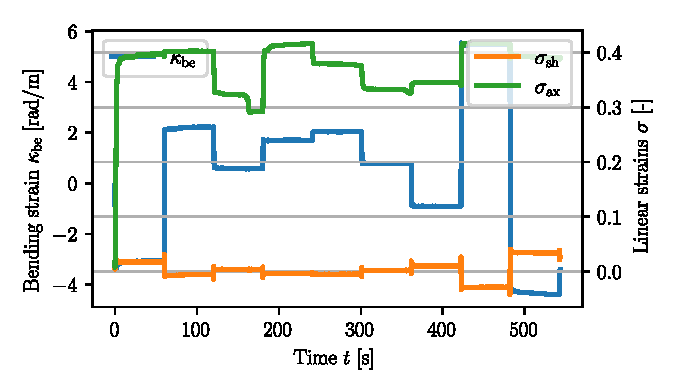
\includegraphics[width=0.47\textwidth, trim={5, 5, 5, 5}]{hsacontrol/figures/experimental_results/task_space_impedance_control/20231030_181558_q.pdf}\label{fig:hsacontrol:experimental_results:task_space_impedance_control:q}}
    \subfigure[Control input $\phi$]{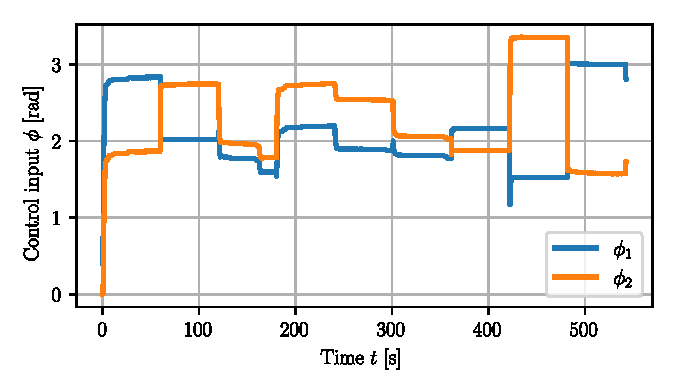
\includegraphics[width=0.47\textwidth, trim={5, 5, 5, 5}]{hsacontrol/figures/experimental_results/task_space_impedance_control/20231030_181558_phi.pdf}\label{fig:hsacontrol:experimental_results:task_space_impedance_control:phi}}
    \caption{Experimental results for tracking a reference trajectory of nine-step functions with the Cartesian impedance controller. \textbf{Panel (a) \& (b):} The x/y-coordinate of the end-effector position with the solid line denoting the actual position, the dotted line the attractor position, and the dashed line the reference (i.e., the setpoint).
    \textbf{Panel (c):} The evolution of the configuration.
    \textbf{Panel(d):} The saturated planar control inputs. }\label{fig:hsacontrol:experimental_results:task_space_impedance_control}
\end{figure}

\subsection{Experimental Setup}
We use the same experimental setup as introduced in Sec.~\ref{sub:hsacontrol:configuration_space_regulation:experimental_setup}.
Over a duration of \SI{540}{s}, we randomly generate nine setpoints $x^\mathrm{d}(t) \in \mathbb{R}^2$ within the operational workspace of the robot (see Fig.~\ref{fig:hsacontrol:kinematics:workspace}).
We evaluate the Cartesian impedance controller using the gains $K_\mathrm{p} = \SI{300}{N \per m}$, $K_\mathrm{d} = \SI{1.5}{N s \per \meter}$ at a frequency of \SI{50}{Hz} and finally send the desired motor positions to the servos.

% \subsection{Evaluation metrics}
% For evaluation purposes, we analyze the response time for reaching the proximity of the setpoint, which we define as $\lVert x^\mathrm{d} - x(t)\rVert_2 \leq \SI{2}{mm}$. Furthermore, we qualitatively assess the transient behavior of the system and the control input $\phi$.

\subsection{Results}
In Fig.~\ref{fig:hsacontrol:experimental_results:task_space_impedance_control}, we present the results of the experimental evaluation of the Cartesian impedance controller. 
The fast response time, a well-known characteristic of model-based control approaches, is evident. However, the errors in the model (for example, caused by hysteresis or unmodeled nonlinearities)~\citep{stolzle2024experimental}, together with the lack of integral action, lead to steady-state errors, which are especially pronounced for the y-coordinate.

